\documentclass{article}
\usepackage[bottom=0.5cm, right=1.5cm, left=1.5cm, top=1.5cm]{geometry}
\usepackage{amsmath}
\usepackage{amssymb}
\usepackage{amsthm}
\usepackage{enumitem}
\usepackage{exercise} % Exercises Style
\usepackage{graphicx}
\usepackage{caption}
\usepackage{environ}
\newenvironment{solution}
{\renewcommand\qedsymbol{$\blacksquare$}
\begin{proof}[Solution]$ $}
  {
\end{proof}}

% Enable Code
\usepackage{minted}
\let \extra T

\newcommand{\vect}[1]{\boldsymbol{#1}}
\newcommand{\E}{\mathbf{E}}
\DeclareMathOperator{\Tr}{Tr}
\DeclareMathOperator{\Cov}{Cov}
\DeclareMathOperator{\Var}{Var}
\DeclareMathOperator{\MSE}{MSE}

\title{Solutions to Assignment 3}
\author{Rongfei Jin}
\begin{document}
\maketitle
\section*{Conceptual 1}
\begin{solution}

  The null hypothesis is the following:
  \(H_0:\beta_0 = 0\) (TV)
  \(H_0:\beta_1 = 0\) (Radio)
  \(H_0:\beta_2 = 0\) (Newspaper)

  Assume we pick \(\alpha = 0.05\) as the significance level.
  Then, the p-value of TV and Radio are both smaller than 0.05, so we reject the null hypothesis and conclude that TV and Radio have significant impact on sales.
  However, the p-value of Newspaper is larger than 0.05, so we fail to reject the null hypothesis and conclude that Newspaper does not have significant impact on sales.

\end{solution}

\section*{Conceptual 3}
\begin{solution}
  \begin{enumerate}[label=(\alph*)]
    \item Let the GPA and IQ be \(c_1,c_2 \in \mathbb Z^* \)
      The model then can be written as:
      \[
        \hat y = 50 + 20c_1 + 0.07c_2 + 35x_3 + 0.01c_1 c_2 -10x_3c_1 + 0.01x_3c_2
      \]
      \begin{enumerate}[label=(\roman*)]
        \item wrong, let \(c_1 = 4\) then \(x_3 = 1\) will result in a smaller predicted value than when \(x_3=0\)
        \item wrong, let \(c_1 = 1\), then \(x_3 = 1\) will result in a greater predicted value than when \(x_3=0\)
        \item right, let \(c_1 = 4\) then \(x_3 = 1\) will result in a smaller predicted value than when \(x_3=0\)
        \item wrong since it is the opposite of (iii)
      \end{enumerate}
    \item substitute the values into the expression above, \(\hat y = 137.1\)
    \item small interaction does not necessary means the interaction is not significant. The significance of the interaction term should be determined by the p-value and the p-value is determined by standard error of the parameter and the parameter itself.
  \end{enumerate}
\end{solution}
\section*{Conceptual 6}
\begin{solution}
  We can substitute the value of \(\bar x\) into (3.4) to get
  \begin{align*}
    \hat y &= \hat \beta_0 + \hat \beta_1 \bar x \\
    &= \bar y - \hat \beta_1 \bar x + \hat \beta_1 \bar x \\
    &= \bar y
  \end{align*}
\end{solution}
\newpage
\section*{Applied 8}
\inputminted{r}{q8.R}[lineos,breaklines]
A linear relationship exists between mpg and horsepower. The p-value of horsepower is less than 0.05, so we reject the null hypothesis and conclude that horsepower has significant impact on mpg. This impact is negative since the coefficient of horsepower is negative. The R-squared is 0.6011, which means 60.11\% of the variation in mpg can be explained by the linear relationship between mpg and horsepower. The strength of the linear relationship is moderate.

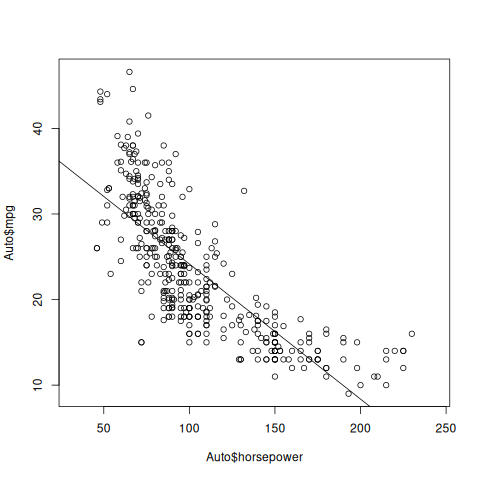
\includegraphics[scale=0.5]{q8.png}
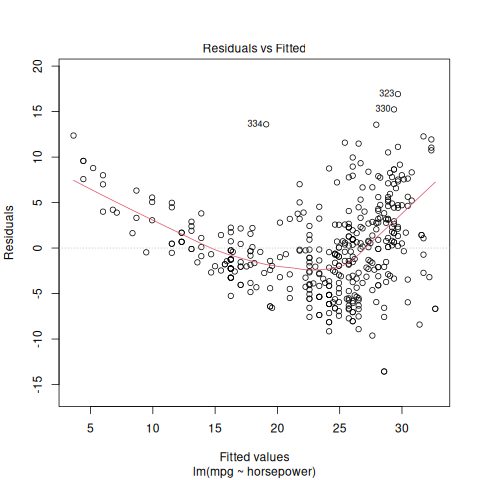
\includegraphics[scale=0.5]{q8_2.png}

The Residual plot at fitted values between 5-20 shows consistent residual variations. However, above 20, the greater variations appear, suggesting that the linear model may not be appropriate for the data above 20.
\newpage

\section*{Applied 9}
\inputminted{r}{q9.R}

\begin{enumerate}[label=(\alph*)]
  \item
    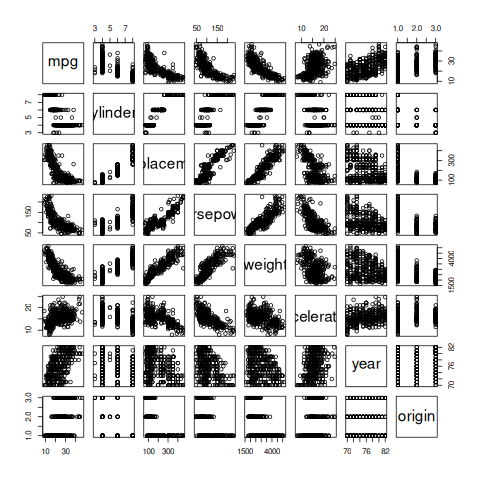
\includegraphics[scale=0.4]{q9.png}

    There exists a relationship between mpg and other predictors. Cylinder, displacement, weights, year and origin are significant predictors. The coefficient of year is poisitive 0.75, indicating that the mpg increases by 0.75 for each additional year.

  \item (See code above)
  \item
    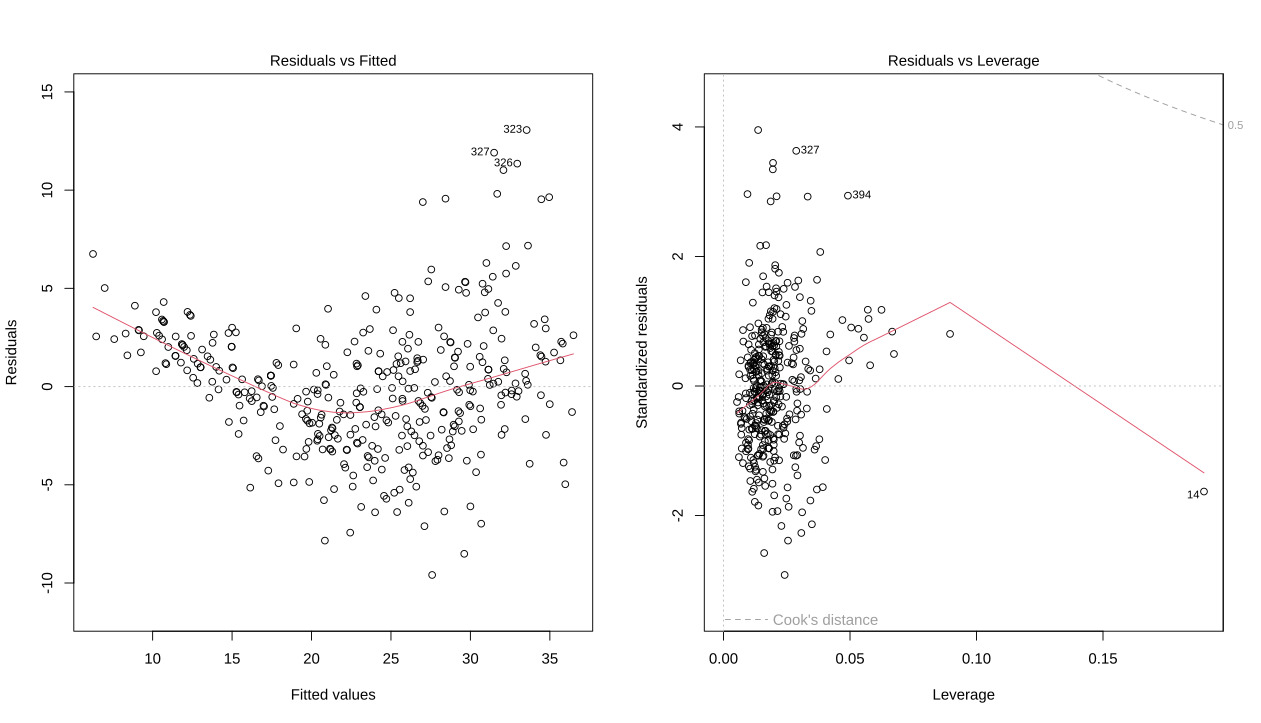
\includegraphics[scale=0.3]{q9_2.jpg}

    The residual plots shows that the distribution of residual is not consistently. So the linear model may not be appropriate for the data.

    The leverage plot shows that there exists 1 extreme outliers and some less extreme outliers

  \item
    The interactions of some predictors, such as cylinders times horsepower, are significant.

  \item
    The transformation fo the response further improves the model by lowering the residual standard errors and increasing the R-squared.

\end{enumerate}
\newpage

\section*{Applied 15}
\inputminted{r}{q15.R}
\begin{enumerate}[label=(\alph*)]
  \item All the predictors except chaos are significant
  \item The multiple linear regression model yields a model with 0.45 R squared. Predictor zn, dis, rad and medv are significant predictors to reject null hypothesis. The coefficient of dis is negative, indicating that the crime rate increases as the distance to employment centers decreases. The coefficient of rad is positive, indicating that the crime rate increases as the accessibility to radial highways increases. The coefficient of medv is negative, indicating that the crime rate decreases as the median value of owner-occupied homes increases.
  \item 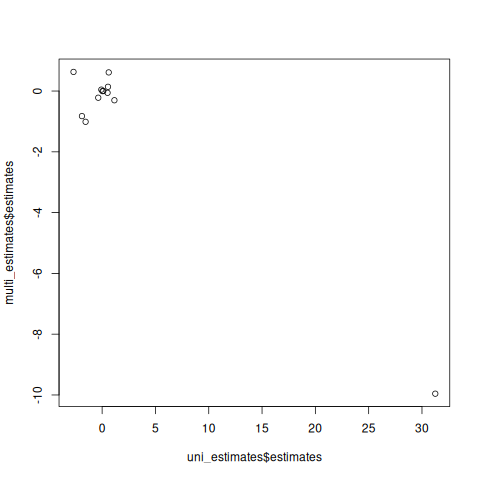
\includegraphics[scale=0.5]{q15.png}

    The estimates from the multiple linear regression model and the stepwise regression model are different especially for the estimator of nox
  \item Some coefficients in polynomial model are significant such as \(x^2, x^3\) of nox, indus and medv, suggesting that the data may be non-linear
\end{enumerate}
\newpage
\section*{Additional 1}
\begin{align*}
  \nabla f(\vect{x}) &=
  \begin{bmatrix}
    \frac{\partial f}{\partial x_1} \\
    \vdots \\
    \frac{\partial}{\partial x_n}
  \end{bmatrix} \\
  &=
  \begin{bmatrix}
    \frac{\partial}{\partial x_1} \vect u^T \vect x\\
    \vdots \\
    \frac{\partial}{\partial x_n} \vect u^T \vect x
  \end{bmatrix} \\
  &=
  \begin{bmatrix}
	\frac{\partial}{\partial x_1} \sum u_i x_i\\
	\vdots \\
	\frac{\partial}{\partial x_n} \sum u_i x_i
  \end{bmatrix} \\
  &= \begin{bmatrix}
	\vect u_1 \\
	\vdots \\
	\vect u_n
  \end{bmatrix} \\
\end{align*}
\section*{Additional 2}

\begin{align*}
	  \nabla f(\vect{x}) &=
  \begin{bmatrix}
	\frac{\partial f}{\partial x_1} \vect x^T \vect A \vect x \\
	\vdots \\
	\frac{\partial}{\partial x_n}\vect x^T \vect A \vect x
  \end{bmatrix} \\
\end{align*}

We take \(x_1\) and the rest will follow

\begin{align*}
	  \frac{\partial f}{\partial x_1} &= \frac{\partial}{\partial x_1} \vect x^T \vect A \vect x \\
  &= \frac{\partial}{\partial x_1} \sum^j\sum^i a_{ij}x_ix_j \\ 
  &= \frac{\partial}{\partial x_1}(\sum_{j=2}^n a_{1j}x_1x_j + \sum_{i=2}^n a_{i1}x_ix_1 + x_1^2a_{11}) + 0\\
  &= \sum_{j=2}^n a_{1j}x_j + \sum_{i=2}^n a_{i1}x_i + 2a_{11}x_1\\
  &= \sum_{j=1}^n a_{1j}x_j + \sum_{i=1}^n a_{i1}x_i\\
  &= 2\sum_{j=1}^n a_{1j}x_j & \text{symmetric property of } A\\
  &= 2(\vect A_{1\cdot} \vect x)
\end{align*}

We can write the rest in a similar way and get the final result
\begin{align*}
  \nabla f(\vect{x}) &= 2 \vect A \vect x
\end{align*}
\newpage
\section*{Additional 3}
From Exercise 2, we know \begin{align*}
  \frac{\partial f}{\partial x_1} &= 2 \sum_{j=1}^n a_{1j}x_j \\
  \frac{\partial^2 f}{\partial^2 x_1} &= 2 \sum_{j=1}^n a_{1j} \\
\end{align*}
\end{document}

